\chapter{Results and Discussion}
\label{cha:results}
\section{Numerical Tests in an 2D Toy Potential}
\label{sec:2D}
For numerical tests the dynamics of a single particle in potential $U_2(x,y)$ (eq. \ref{eq:U2}) is simulated under application of different biasing algorithms.
Including both the $x$ and $y$ direction the full configuration space is used as CV space.
The analytical PMF and free energy difference is therefore given by
\begin{equation}
  \begin{split}
    A(x,y)&=U_2(x,y) \\
    \Delta A_{A\to B} &= 0
  \end{split}
\end{equation}
The convergence of numerical calculations of PMFs to the analytical result with different adaptive biasing schemes (MtD, WTM, ABF, eABF and WTM-eABF) is computed in 5~ns trajectories.
Note that all adaptive biasing methods depend on a different set of parameters.
Their convergence can therefore only be compared qualitatively.
A detailed analysis of the impact of the choice of parameters will be given in the following section.
Parameters applied in this section are given in table~\ref{tab:2D params} of the appendix.
The conference of the analytical PMF and the development of free energy differences $\Delta A_{A\to B}$ is given in figure~\ref{fig:conv 2D}.
Figure~\ref{fig:error 2D} shows the absolute errors of the obtained PMFs after 5~ns.
Additional snapshots of the numerical PMF at 1, 3 and 5~ns are given in the appendix.
\begin{figure}[H]
   \centering
   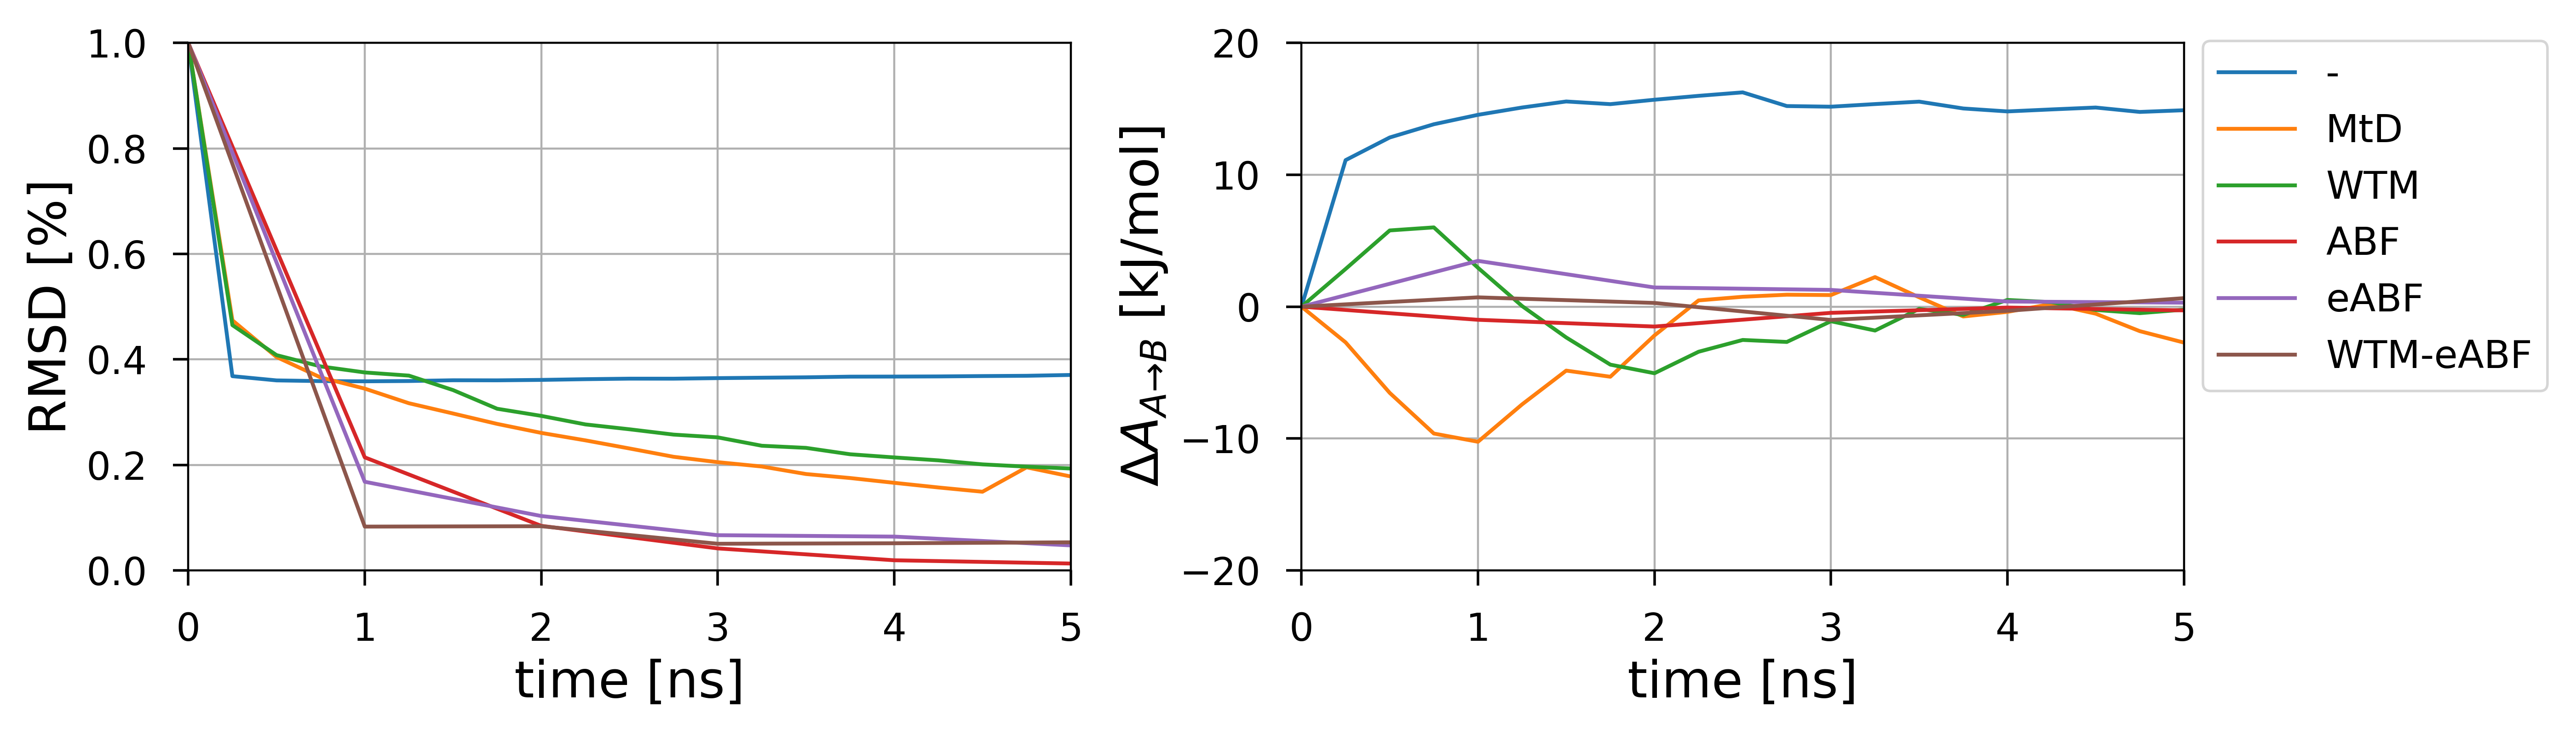
\includegraphics[width=0.99\textwidth]{bilder/test_2D/conv}
   \caption{Convergence of free energy calculations with different adaptive biasing methods for 2D toy potential $U_2(x,y)$. On the right the RMSD between the analytical and numerical PMF is given over the course of 5~ns trajectories. On the right the development of free energy differences $\Delta A_{A\to B}$ between both minima given by eq.~\ref{eq:free energy diff} is shown. The transition barrier between both minima is on the line $0.25x+y$. Therefore $A$ includes all states $x>-4y$ and $B$ all states $x<-4y$, respectively. Details are given in the appendix.}
 \label{fig:conv 2D}%
 \end{figure}
\begin{figure}[H]
  \centering
  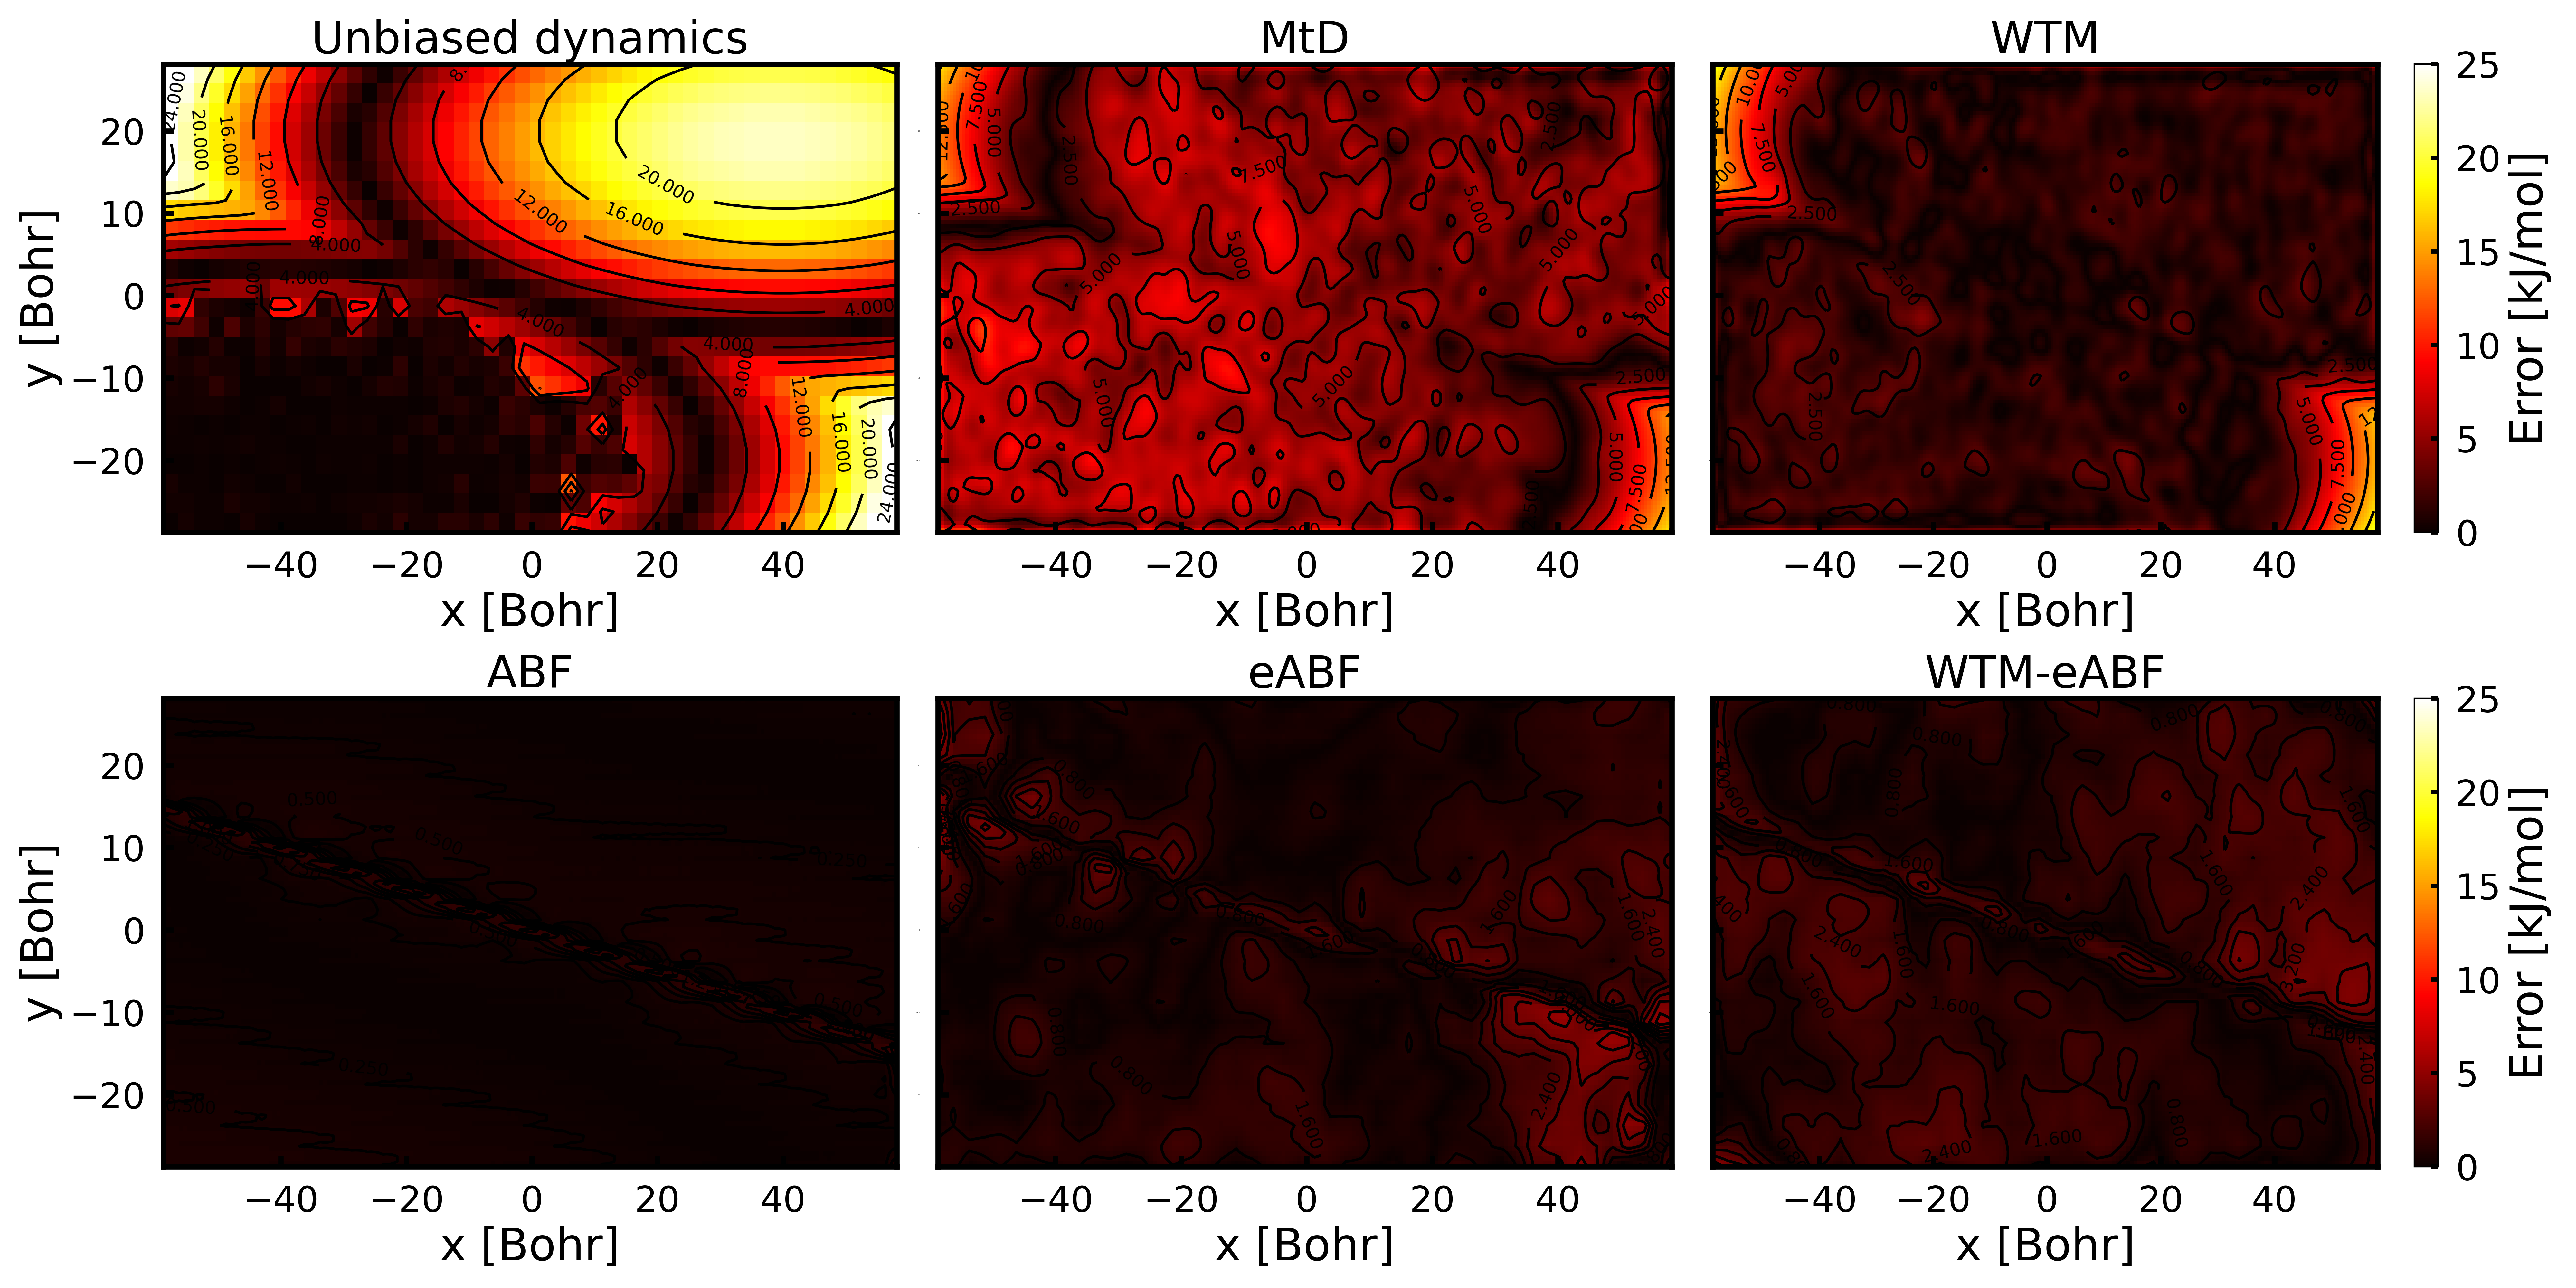
\includegraphics[width=0.99\textwidth]{bilder/test_2D/error_5ns}
  \caption{Heat maps of the absolute difference between the analytic PMF and PMFs computed from 5~ns trajectories at 300~K with different adaptive biasing schemes (Error$=|U_2(x,y)-A_{5ns}(x,y)|$). Details are given in the appendix.}
\label{fig:error 2D}%
\end{figure}
In an unbiased simulation the system stays trapped in one metastable state.
This is a prototypical example of quasi-nonergodic behavior, where simple time averages over MD trajectories do not converge to the correct ensemble average.
Because only one free energy minimum is explored the free energy difference $\Delta A_{A\to B}$ is highly overestimated.

All adaptive biasing methods reduce the metastability significantly and enable uniform sampling of both states.
In metadynamics simulation the PMF is estimated by a superposition of gaussian hills which are deposited linearly over time.
This is reflected by the linear convergence of MtD over time, which strongly depends on the applied parameters.
For this particular set of parameters no complete convergence is not reached after 5~ns.
Therefore some regions at the margin with high free energy remain unexplored, but also in areas that are already filled with gaussians the obtained PMF is characterized by large fluctuations of up to 5~kJ/mol.
By scaling down the gaussian height over time WTM reduces this fluctuations significantly and enables rigorous convergence of the resulting PMF.
This enables rigorous convergence of the free energy difference $\Delta A_{A\to B}$.
However, large local errors in high free energy regions due to incomplete filling of the PMF with Gaussian hills still result in a similar RMSD to the analytical PMF than obtained with MtD.






\newpage
\section{Benchmark Calculations for the Torsion of Cl-F-Ethane}
\label{sec:test}
The following section will give a detailed discussion on the effect of different parameters on the time convergence of adaptive biasing force methods (ABF, eABF and WTM-eABF).
As test system the transition of the dihedral angle between the Cl- and F-group in Cl-F-Ethane from the gauge$^+$ ($60^\circ$) to the gauge$^-$ ($-60^\circ$) structure on the PBEh-3c/dev2-msvp level of theory in vacuum will be considered.

Figure~\ref{fig:ABF benchmark} shows the PMF obtained from a ABF calculation for growing values of $N_{full}$ from 50~ps long trajectories.
Convergence rates will be calculated in reference to the ABF ($N_{full}=100$) result after 50~ps.
After roughly 30~ps all three simulations converge to the same result.
For higher values of $N_{full}$ it takes longer to fill the ramp functions.
Diffusion to other minima along the reaction coordinate and its uniform sampling is therefore delayed and convergence slowed down.
In this particular example, even the unrestrained application of the ABF force from the start ($N_{full}=1$) does not lead to any non-equilibrium effects.
However, as instantaneous force samples depend on all molecular coordinates, the variance of fluctuations in ABF estimates can be expected to grow with the system size.
More specifically fluctuations of the ABF force will be dominated by high frequency terms due to bonded interactions\autocite{lesage2017smoothed}, which also leads to a dependence of the variance in ABF force samples at the beginning of the simulation on the amount of equillibration.\autocite{blondel2004ensemble}
Using smaller values of $N_{full}$ is therefore associated with a certain risk to drive the system away from thermal equilibrium at the beginning of the simulation.
Correcting wrong force estimates obtained with high statistical weight at the beginning of the simulation takes exceedingly long which makes corresponding free energy estimates prone to errors.\autocite{comer2015adaptive}
Overall $N_{full}=100$ is found to result in a good compromise between save and fast convergence of the ABF force estimates for all systems considered in this work.
\begin{figure}[H]
    \centering
    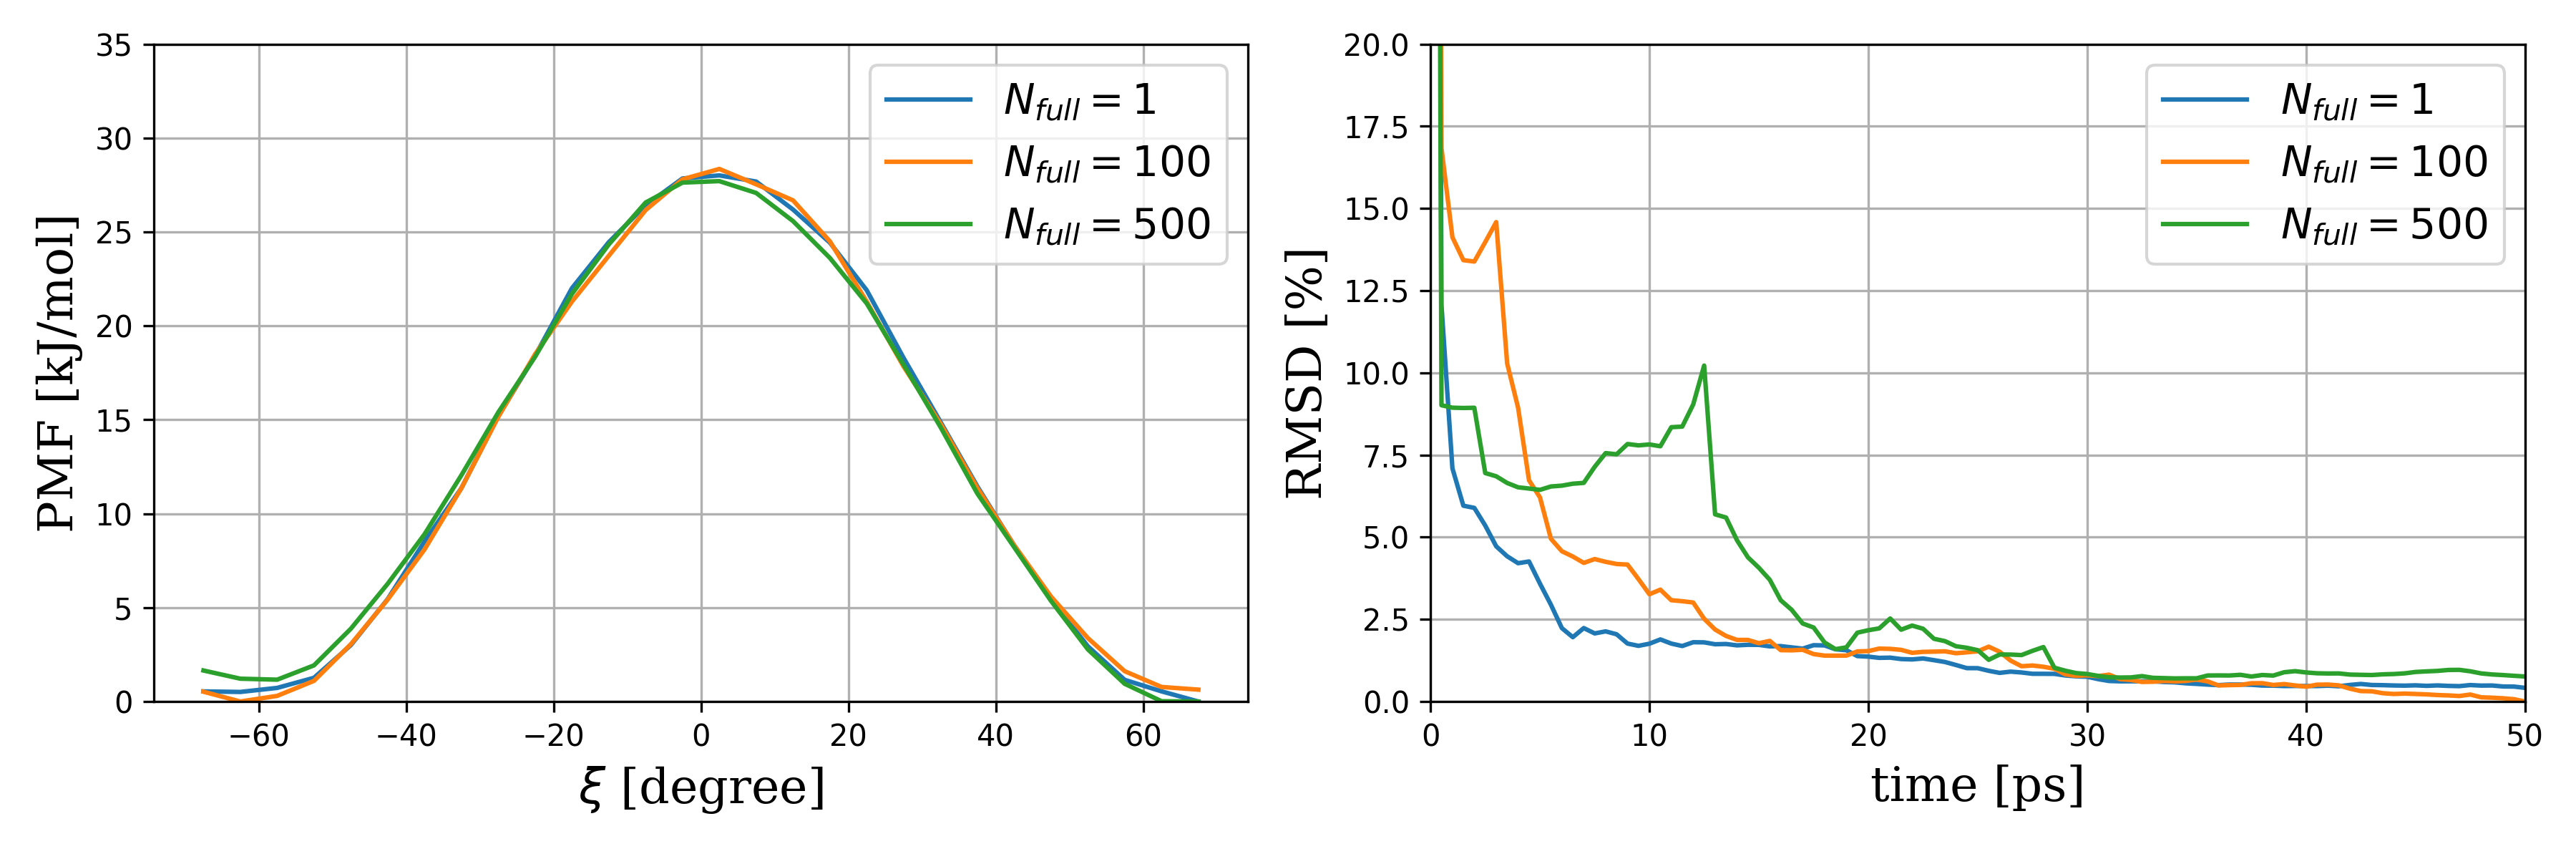
\includegraphics[width=0.99\textwidth]{bilder/benchmark/ABF_benchmark_nfull}
    \caption{ABF benchmark}
    \label{fig:ABF benchmark}
\end{figure}
For eABF the ramp function is applied in the exact same way and with the same consequences than for ABF.\autocite{lesage2017smoothed}
However, mean square fluctuations $\sigma_F$ of the eABF force only depend on the spring force between the CV and the extended variable and is therefore proportional to the harmonic force constant $k_\lambda$.
\begin{equation}
    \sigma_F^2 \propto \frac{k_\lambda}{\beta} = \frac{1}{\beta\sigma_\lambda}
\end{equation}
This implies that in eABF calculations higher the variance of
\begin{figure}[H]
  \centering
    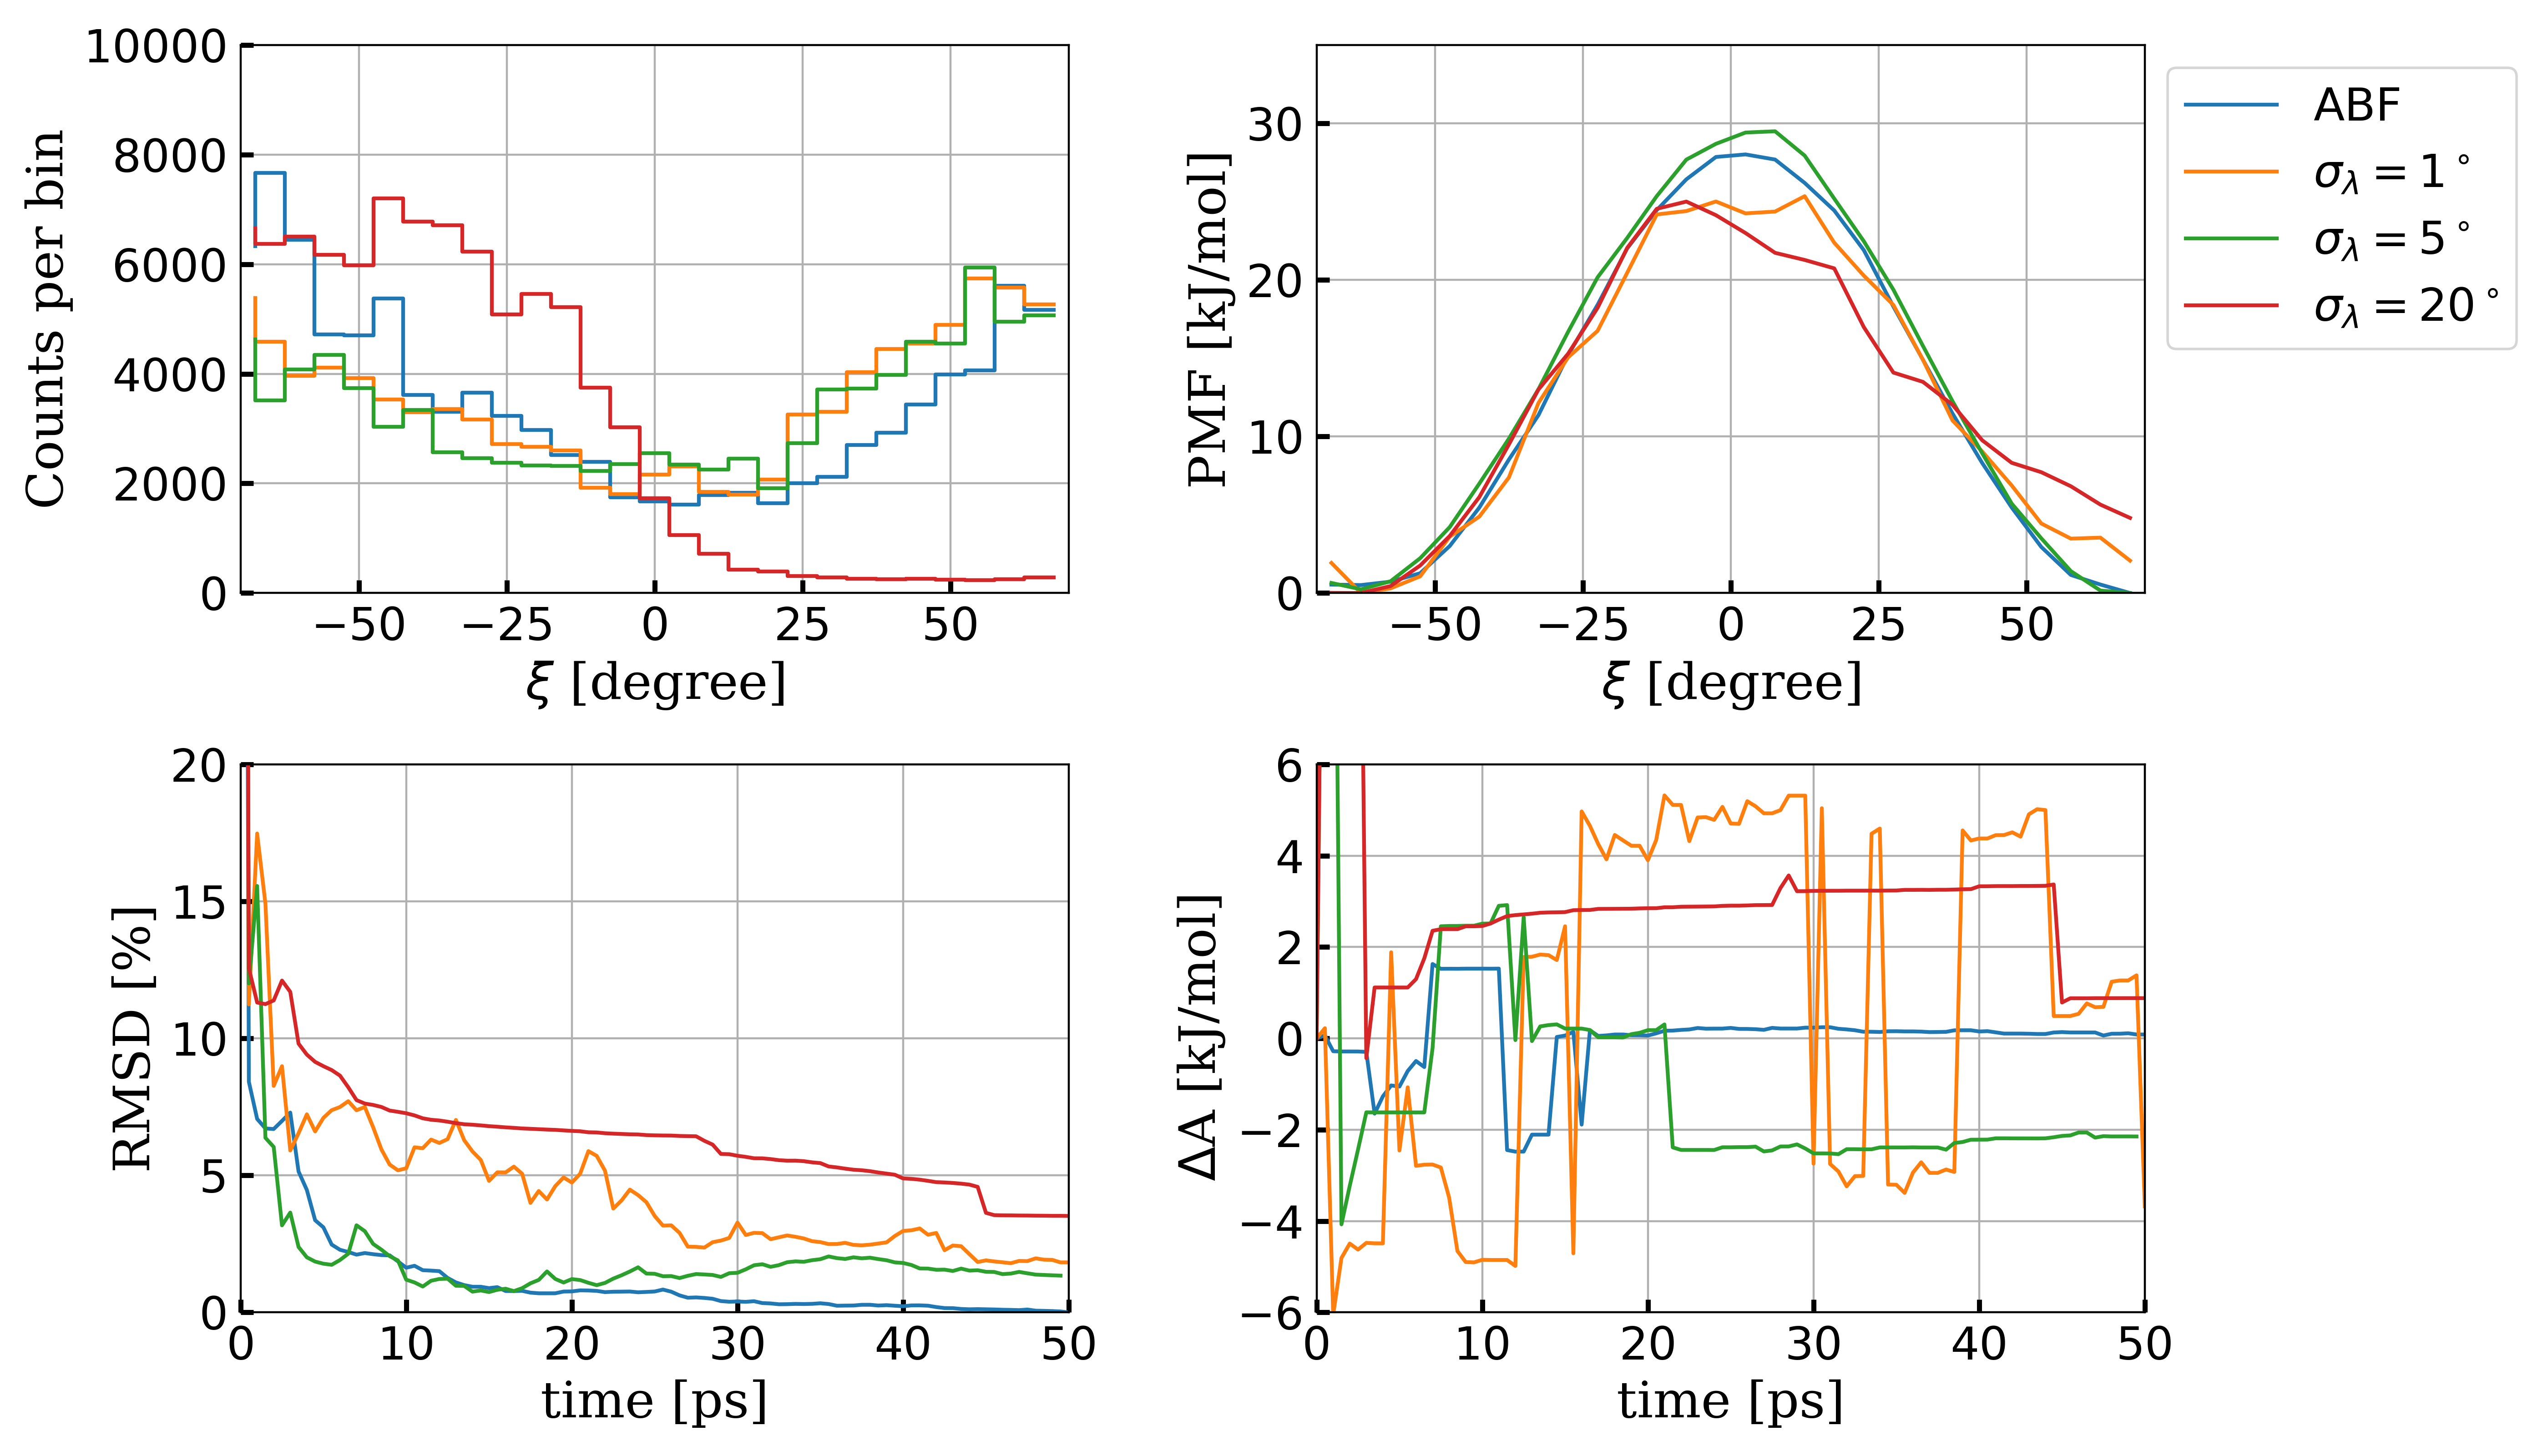
\includegraphics[width=0.99\textwidth]{bilder/benchmark/eABF_benchmark_sigma}
   \caption{Convergence of eABF with $m_\lambda=15$~a.u. and $N_{full}=100$.}
   \label{fig:conf eABF sigma}
\end{figure}

\begin{figure}[H]
  \centering
    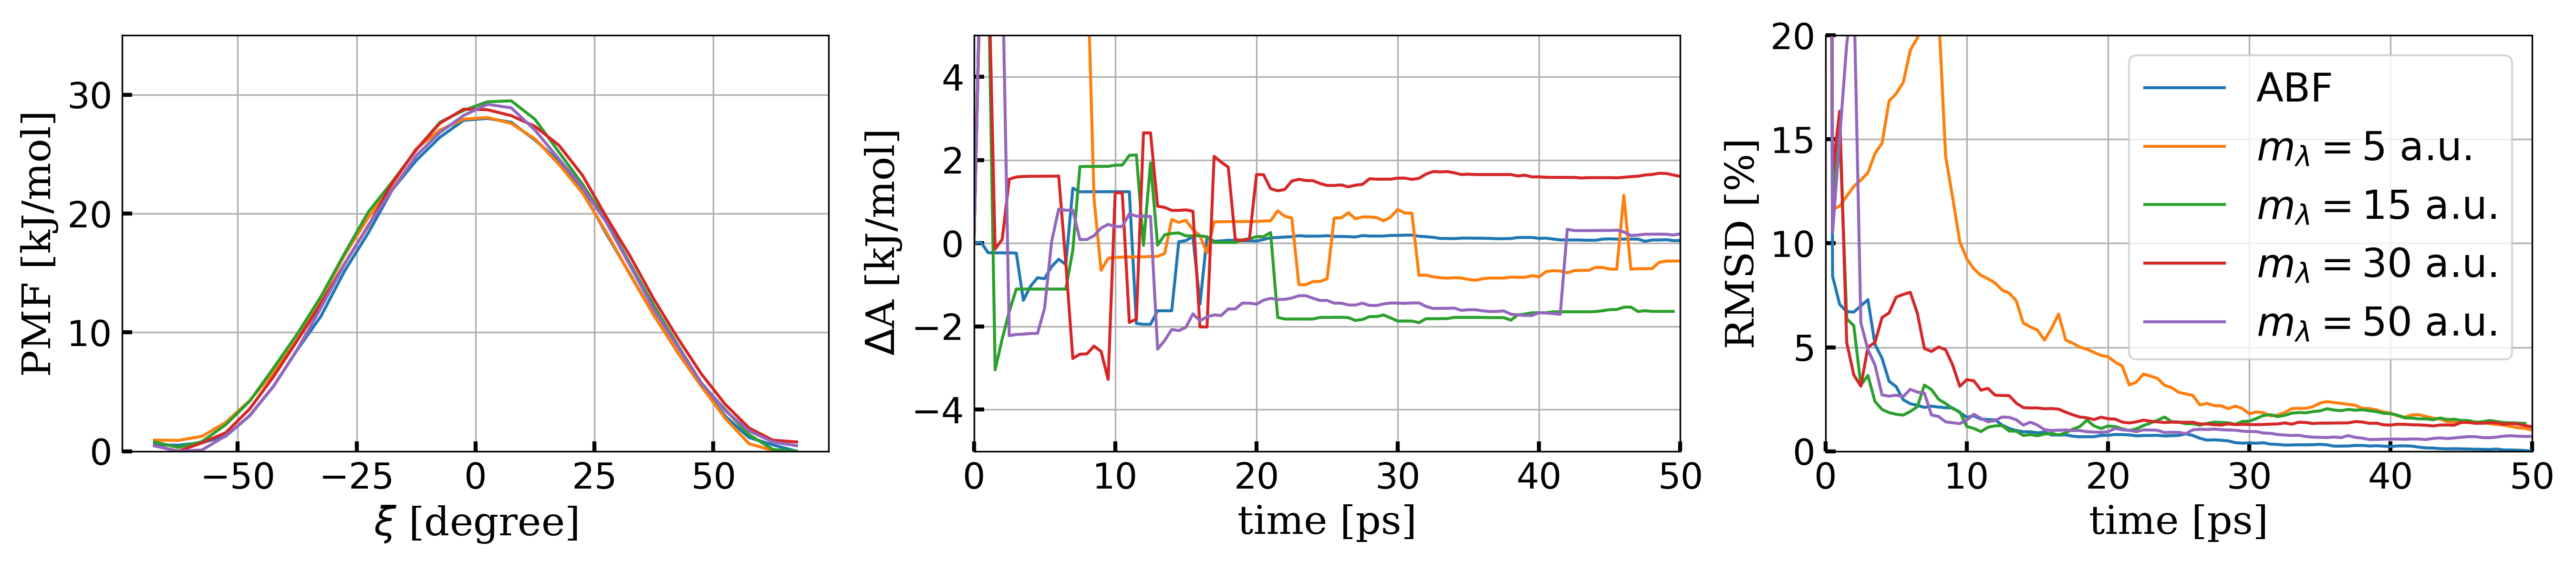
\includegraphics[width=0.99\textwidth]{bilder/benchmark/eABF_benchmark_mass}
   \caption{Convergence of eABF with $\sigma_\lambda=5$ degree and $N_{full}=100$.}
   \label{fig:conf eABF mass}
\end{figure}

\begin{figure}[H]
  \centering
    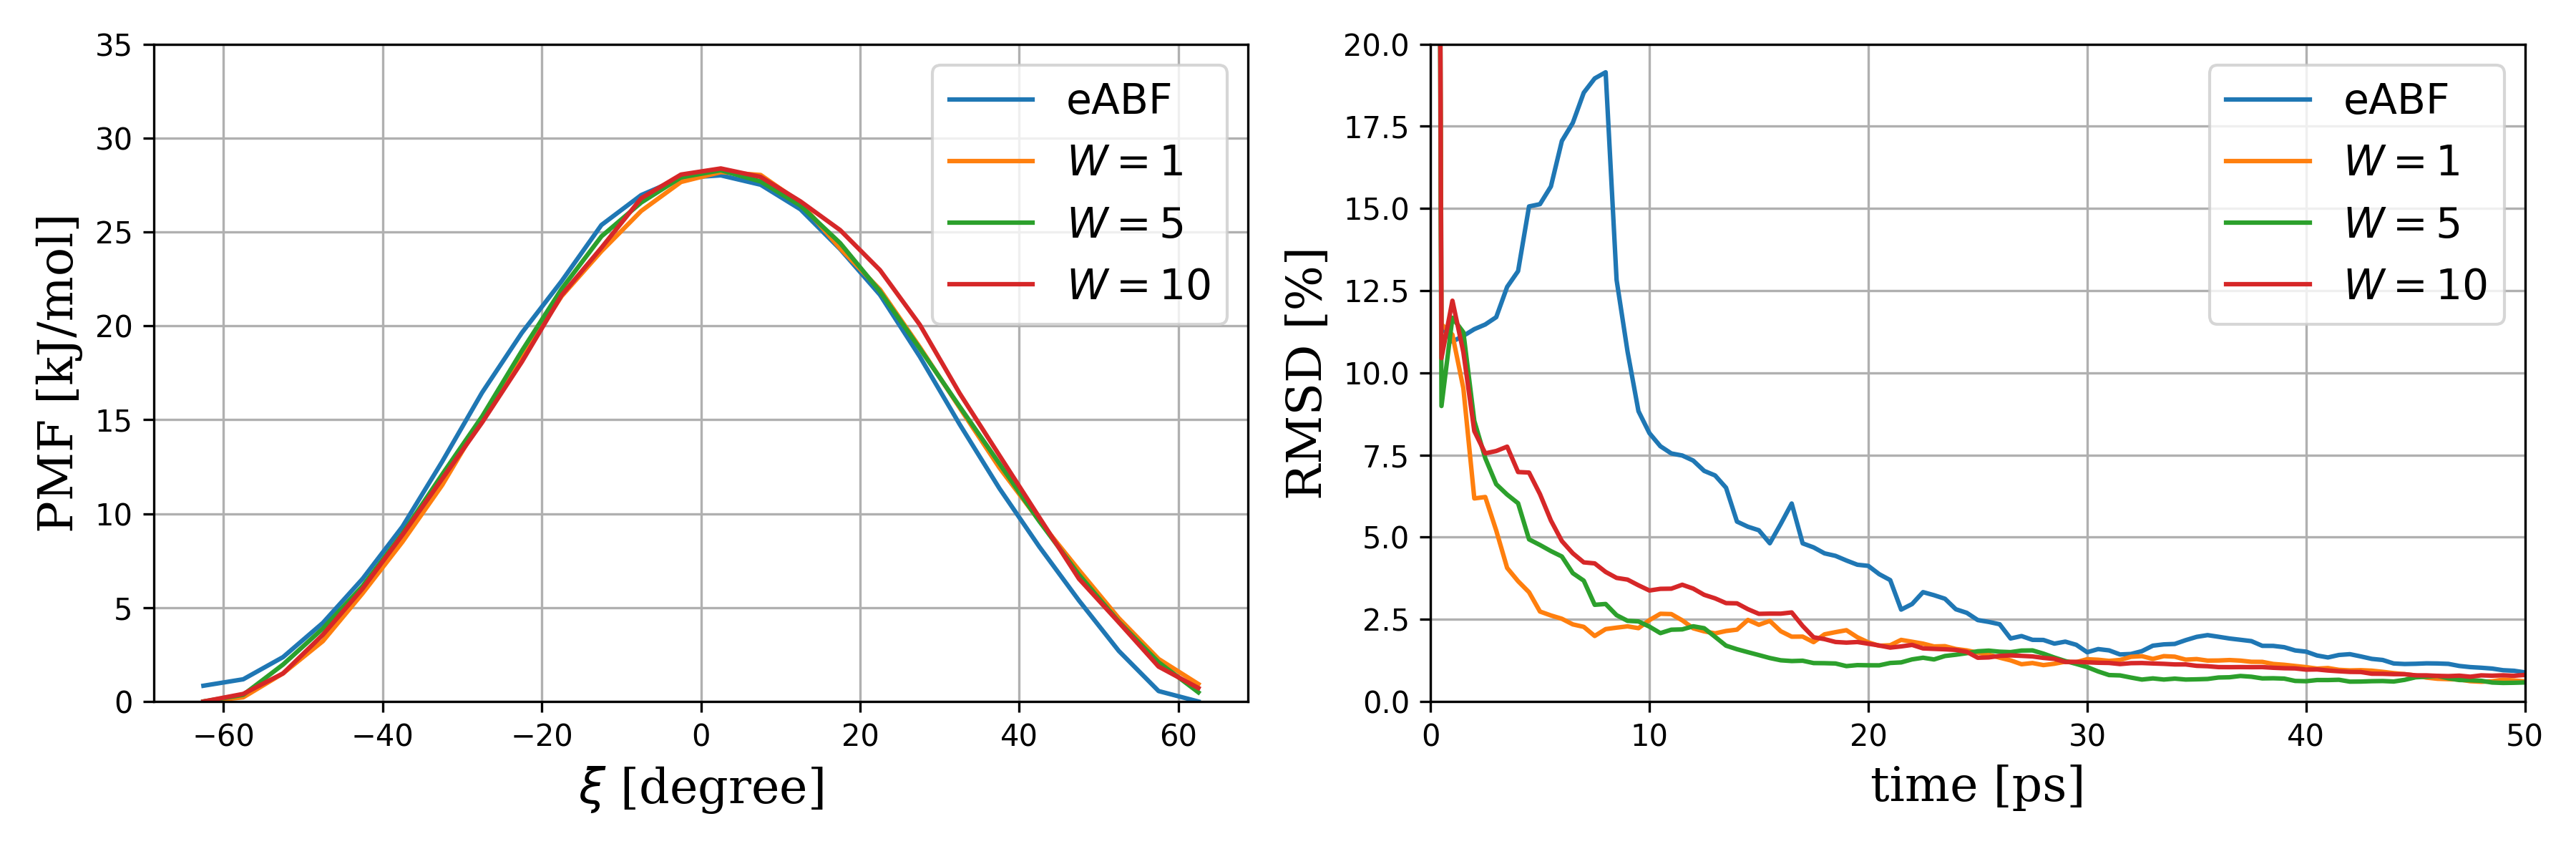
\includegraphics[width=0.99\textwidth]{bilder/benchmark/meta_eABF_benchmark_height}
   \caption{Convergence of WTM-eABF with $m_\lambda=5$~a.u., $\sigma_\lambda=5$, $\sigma_G=5$, $\tau_G=10$~fs, $\Delta T=2000$~K and $N_{full}=100$.}
   \label{fig:conf meABF height}
\end{figure}

\begin{figure}[H]
  \centering
    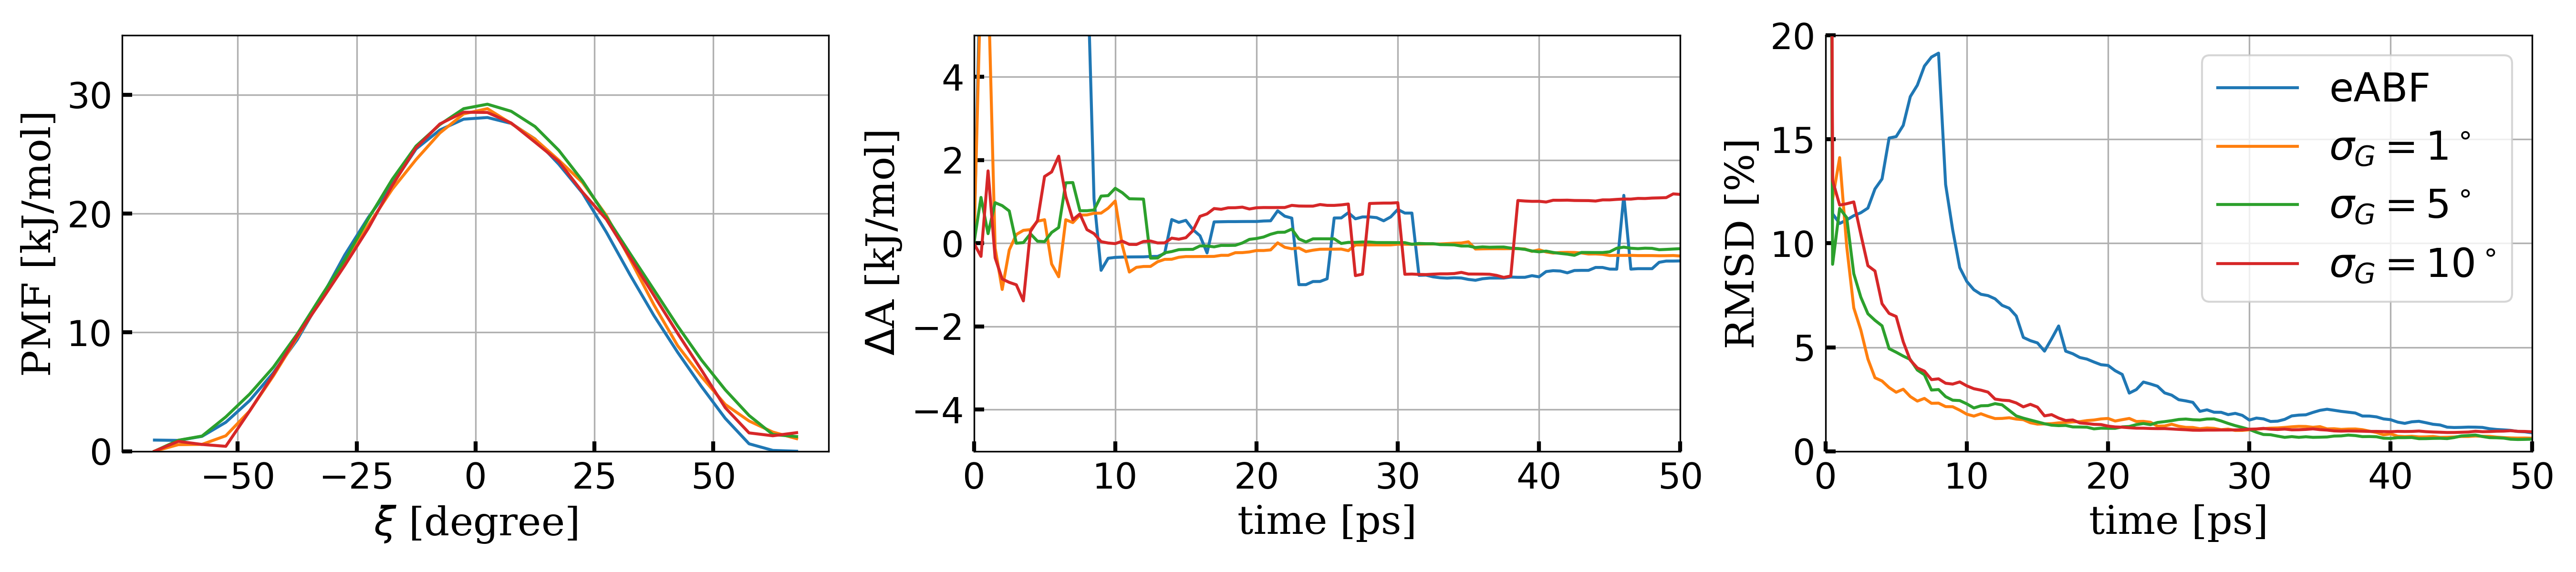
\includegraphics[width=0.99\textwidth]{bilder/benchmark/meta_eABF_benchmark_var}
   \caption{Convergence of WTM-eABF with $m_\lambda=5$~a.u., $\sigma_\lambda=5$, $W=5$ kJ/mol, $\tau_G=10$~fs, $\Delta T=2000$~K and $N_{full}=100$.}
   \label{fig:conf meABF var}
\end{figure}

% \begin{figure}[H]
%     \centering
%     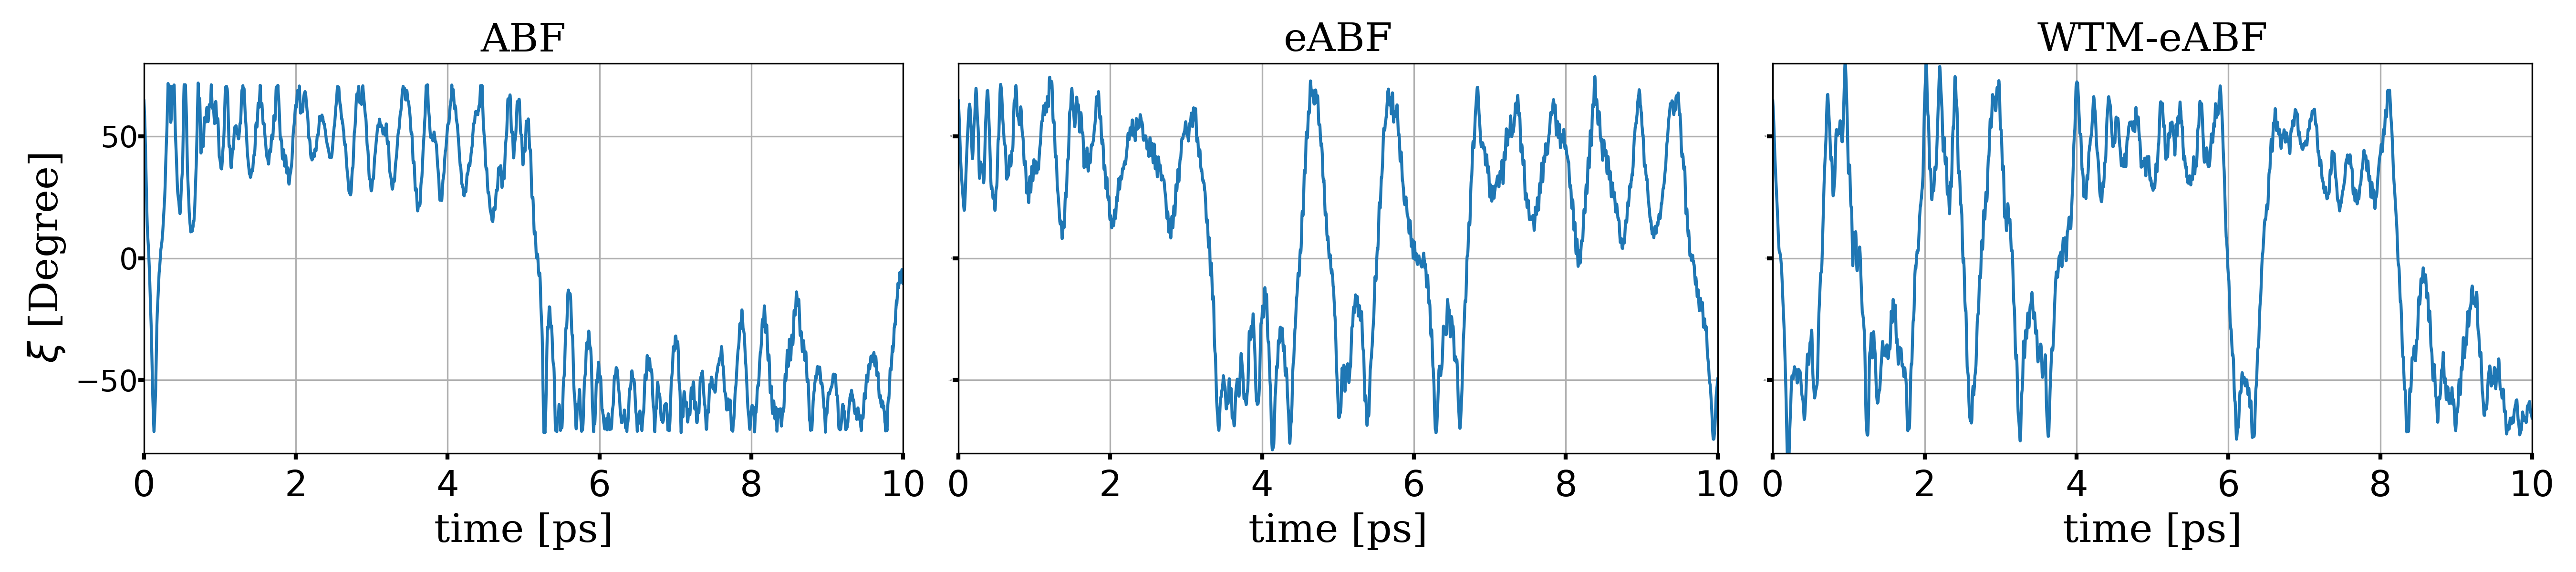
\includegraphics[width=0.99\textwidth]{bilder/benchmark/ABF_trajs}
%     \caption{Trajectories during ABF, eABF and WTM-eABF simulation.}
%     \label{fig:traj ABF}
% \end{figure}

\begin{figure}[H]
  \centering
    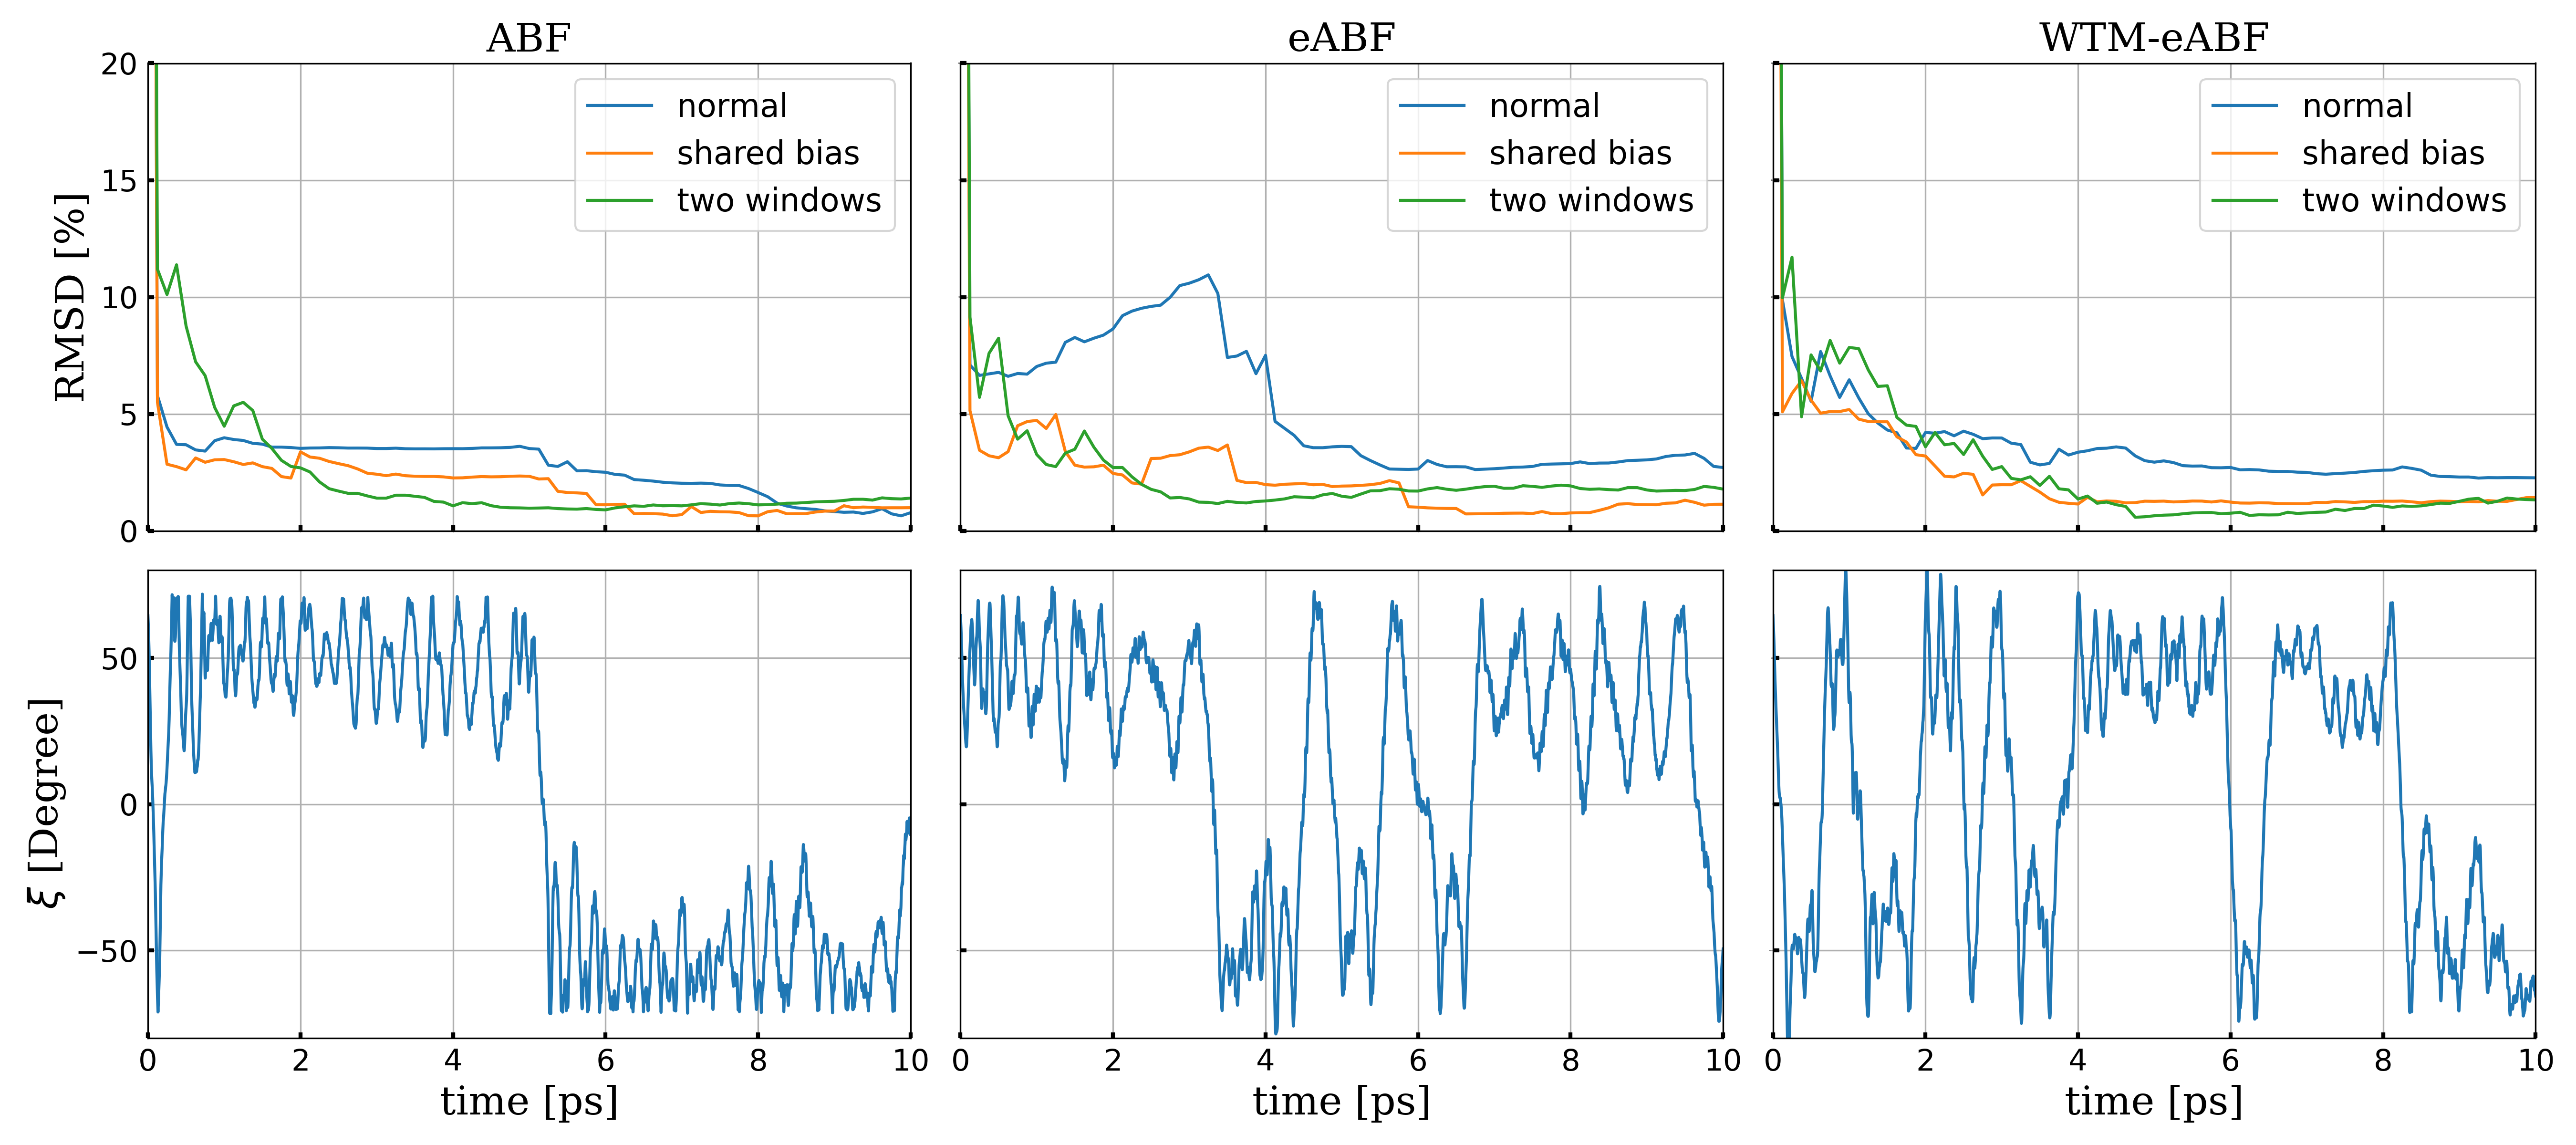
\includegraphics[width=0.99\textwidth]{bilder/benchmark/ABF_acc_benchmark}
   \caption{Convergence of ABF, eABF and WTM-eABF}
   \label{fig:conf ABF}
\end{figure}


% \begin{figure}[H]
%    \centering
%     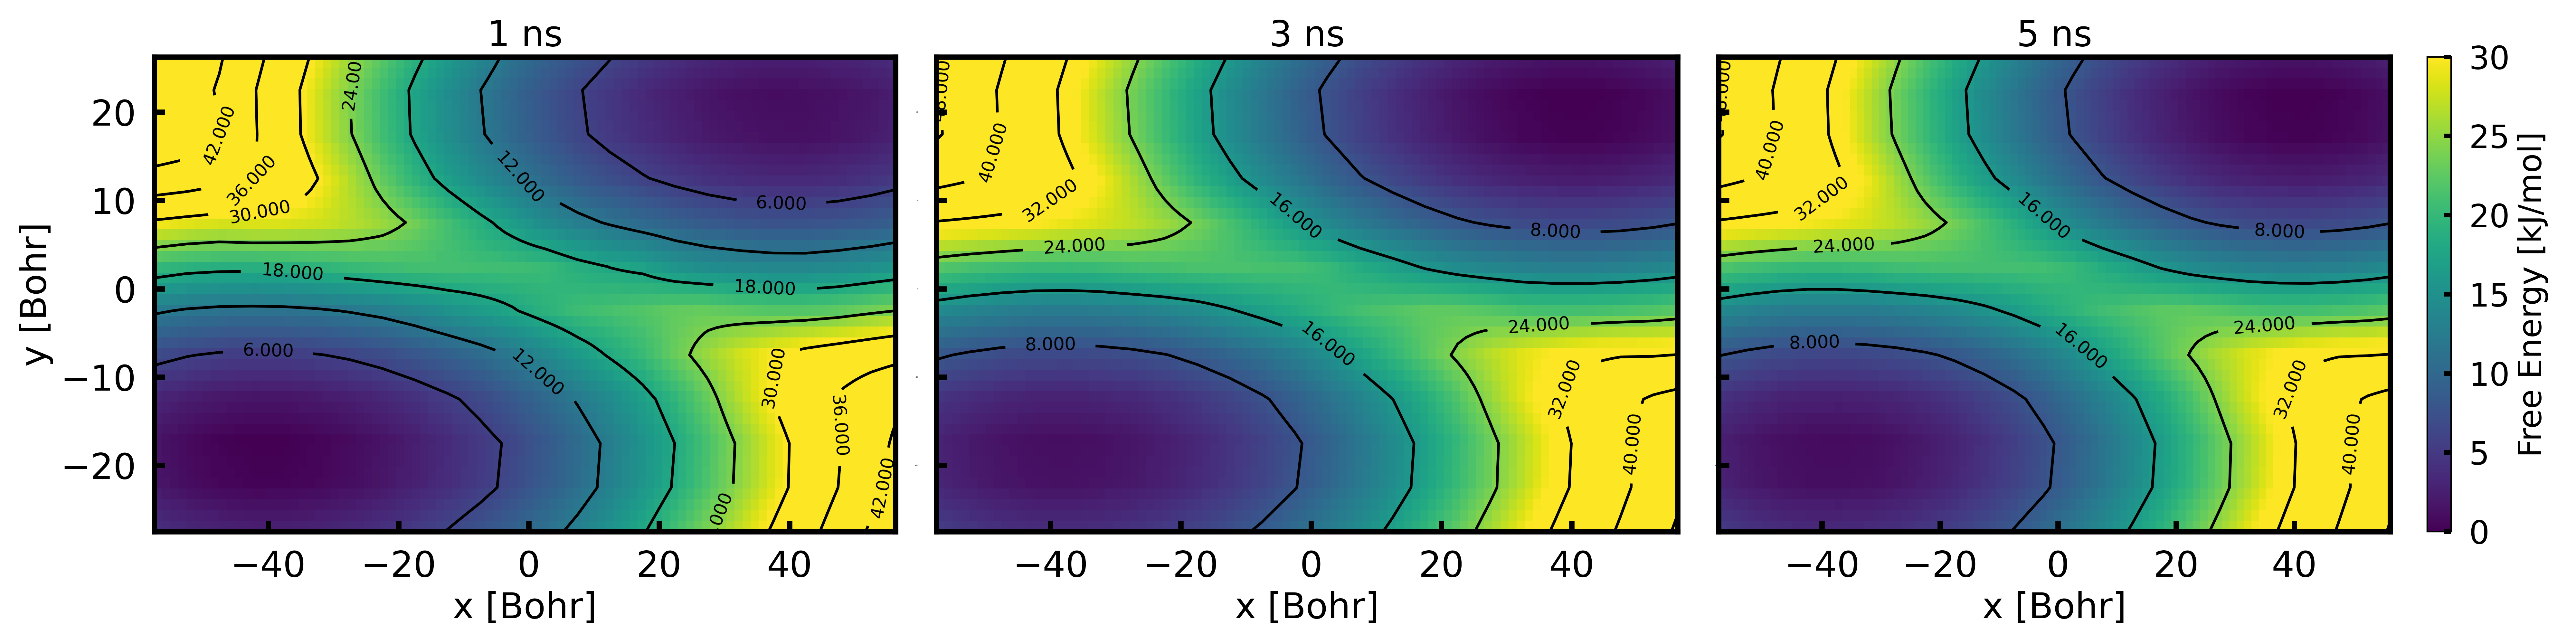
\includegraphics[width=0.99\textwidth]{bilder/test_2D/ABF}  \\
%     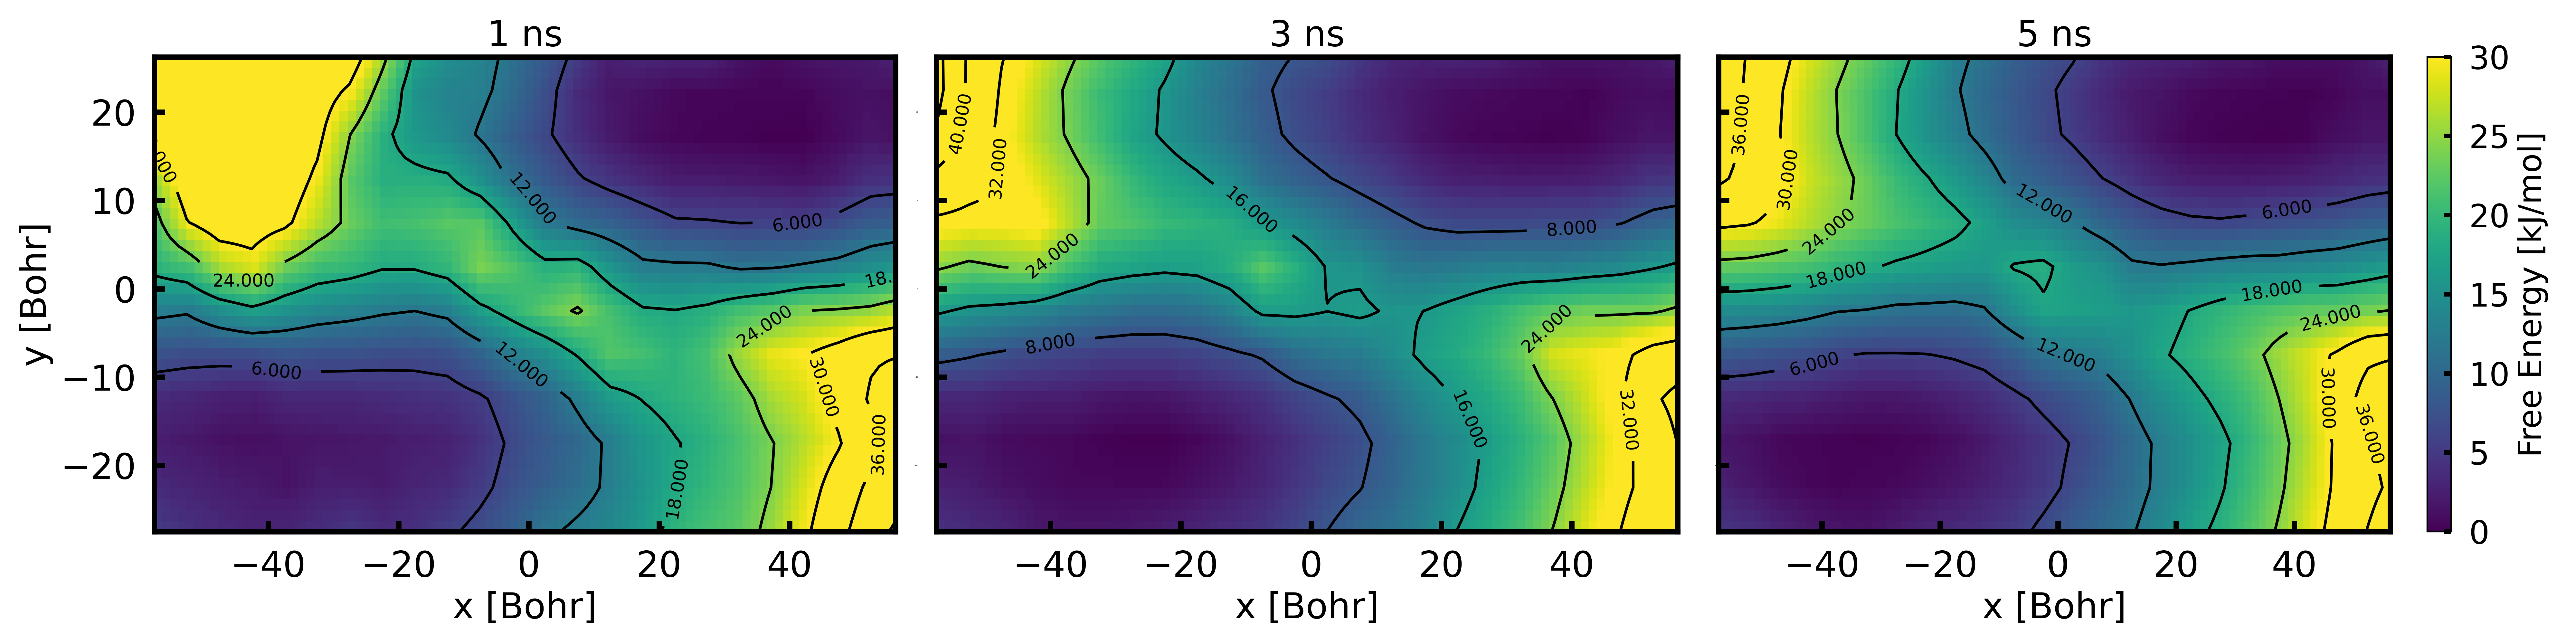
\includegraphics[width=0.99\textwidth]{bilder/test_2D/eABF} \\
%     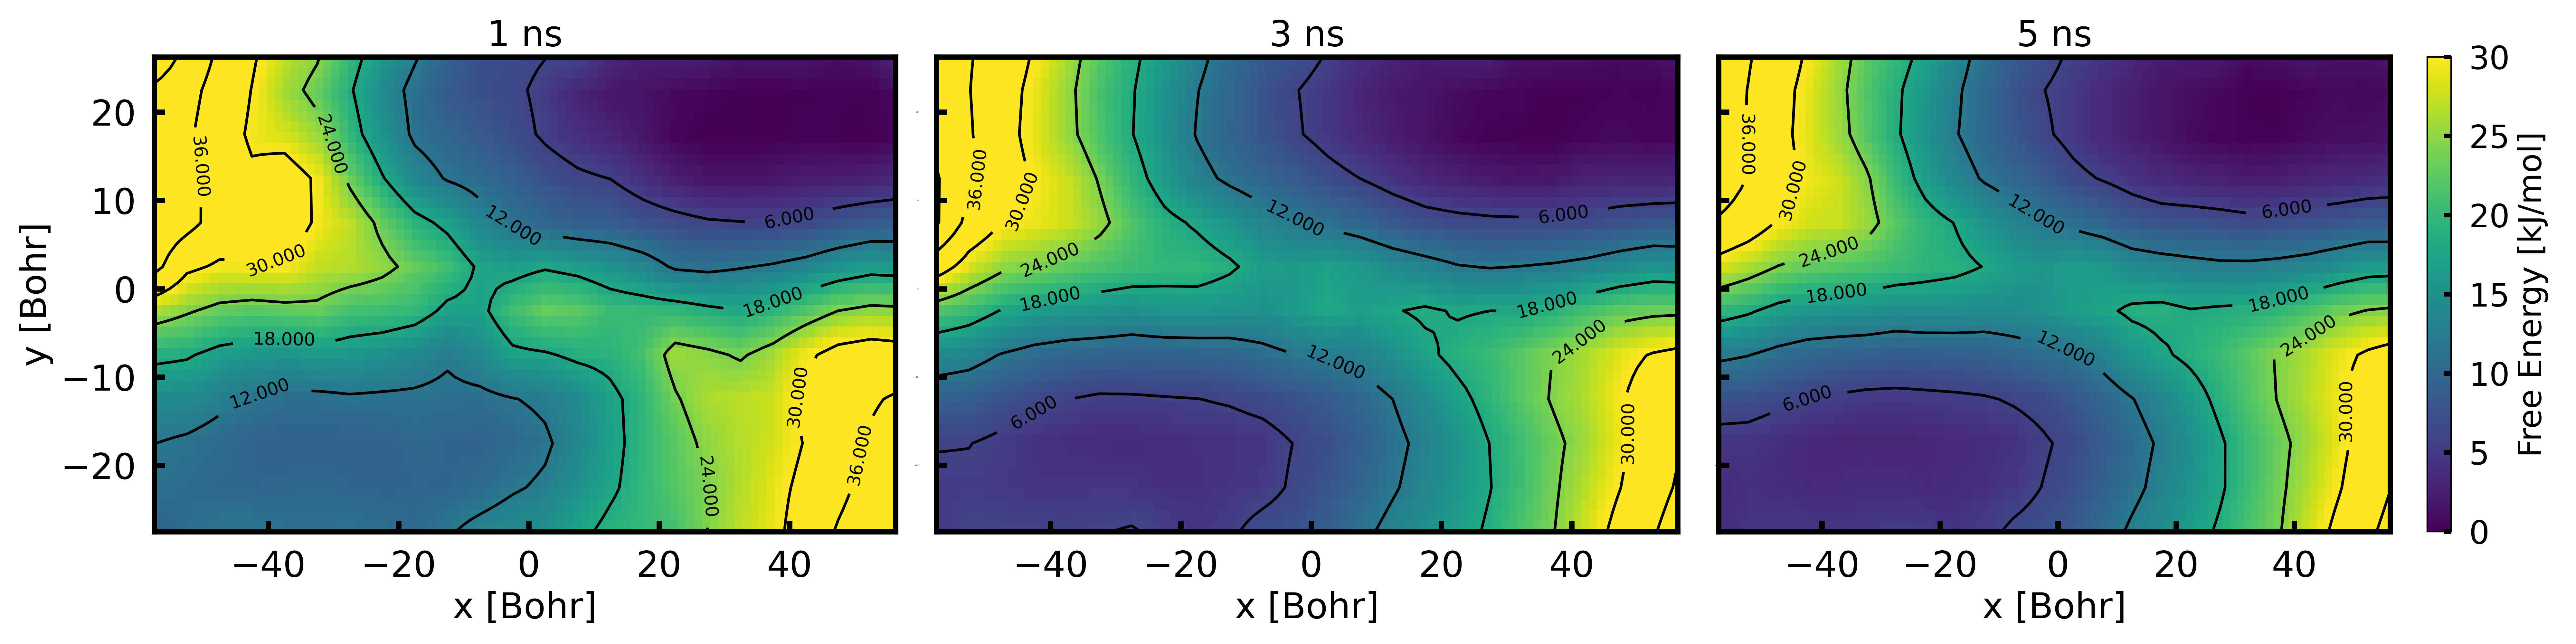
\includegraphics[width=0.99\textwidth]{bilder/test_2D/meta_eABF}
%     \caption{2D ABF, eABF and WTM-eABF test}
% \label{fig:2D ABF}%
% \end{figure}


\section{Application of WTM-eABF to S\textsubscript{n}2-Reactions}
\label{sec:Sn2}


\section{Ring Closing Reaction}
\label{sec:RCR}

\begin{figure}[H]
  \centering
    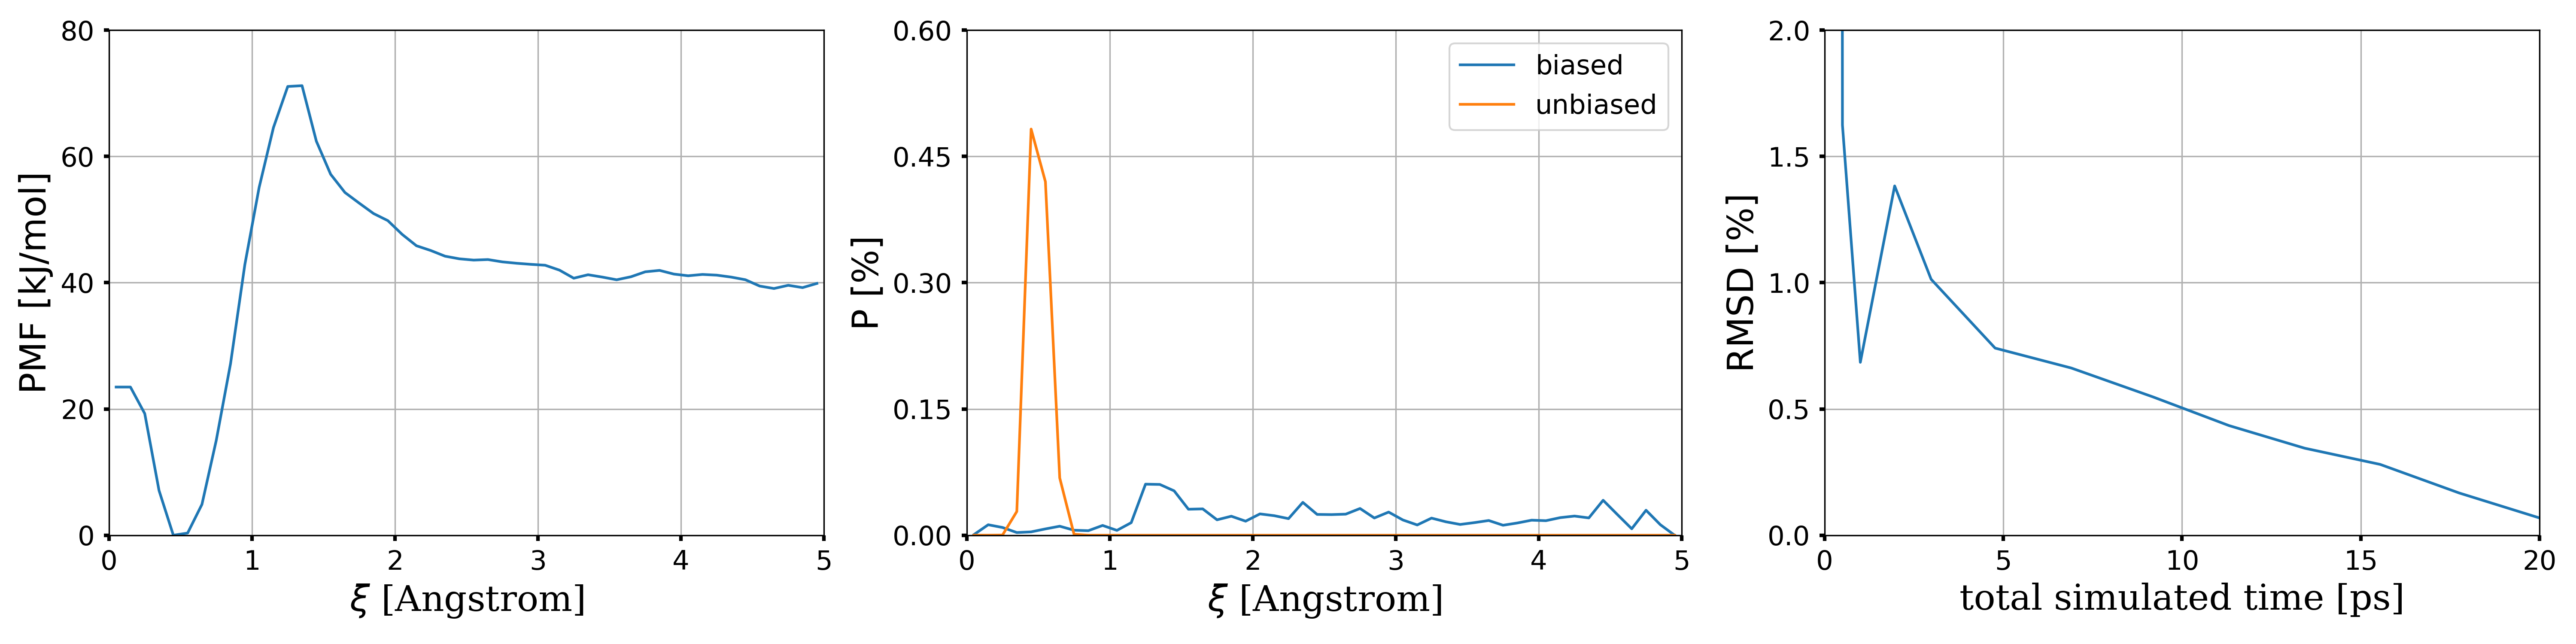
\includegraphics[width=0.99\textwidth]{bilder/results/R2_ool_results}
   \caption{Ring closing reaction}
   \label{fig:ool}
\end{figure}
